
\section{Motivation} \label{sec:motivation}
Data center energy efficiency has become of crucial importance in recent years due to its high economic, environmental, and performance impact. For example, the leading petaflop supercomputers consume a range of 1–18 MW of electrical power, with 1.5 MW on average, which can be easily translated into millions of dollars per year in electricity bills \cite{Group2012HandbookSahni}.
Data center energy consumption was estimated to be between 1.1\% and 1.5\% of worldwide electricity usage in 2010 \cite{Dayarathna2016DataSurvey,Corcoran2017EmergingICT}, generating as much pollution as a nation such as Argentina  \cite{Mathew2012Energy-awareNetworks}.
In some cases, the power costs exceed the cost of purchasing hardware~\cite{Rivoire2007ModelsOptimizations}.
Furthermore, the energy costs of powering a typical data center doubles every five years~\cite{Buyya2013Introduction}.
Therefore, with such a steep increase in power use, electricity bills have become a significant expense for today's data centers \cite{Poess2008EnergyCenters,Gao2013QualityCenters}. 
For these reasons, data center energy efficiency is now considered a primary concern for data center operators, often ahead of the traditional considerations of availability and security.

There are several approaches for green computing, from electrical materials to circuit design, systems integration, and software. These techniques may differ, but they share the same goal---to substantially reduce overall system energy consumption without a corresponding negative impact on delivered performance.
The processor and main memory are  the components that usually dominate power consumption, as shown in \cref{fig:powerbreakdown}.
The processor can consume as much as 50\% of the total energy~\cite{Fan2007PowerComputer, Barroso2007TheComputing, Malladi2012TowardsDRAM}. For that reason, modern processors incorporate several features for power management~\cite{Rotem2012Power-managementBridge, Brown2005ACPILinux, Hackenberg2015AnProcessor, Intel20200thLake}, such as dynamic power management (DPM) and dynamic voltage and frequency scaling (DVFS). 
DPM encompasses a set of techniques for obtaining energy-efficient computing by deactivating or reducing the system components' performance when they are idle or partially utilized~\mbox{\cite{Shuja2012Energy-efficientCenters, Benini2000AManagement}}.
DVFS allows the frequency and voltage to be adjusted in run-time depending on current needs.


\begin{figure}[H]
	\centering
	\captionsetup[subfigure]{justification=centering}
	
	\begin{subfigure}[b]{0.45\textwidth}
		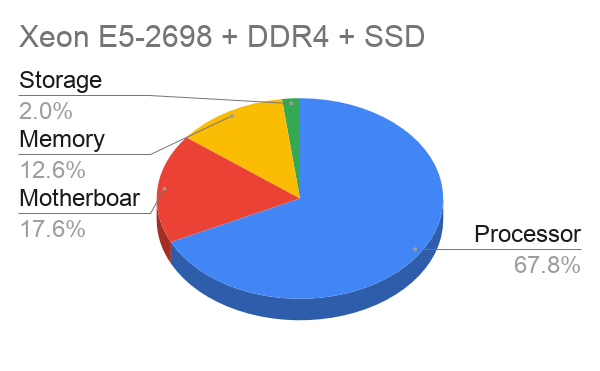
\includegraphics[width=\textwidth]{models/figures/power_breakdown/Xeon E5-2698 + DDR4 + SSD.png}
		\caption{}
		\label{fig:powerbreakdown_a}
	\end{subfigure}
	%
	\begin{subfigure}[b]{0.45\textwidth}
		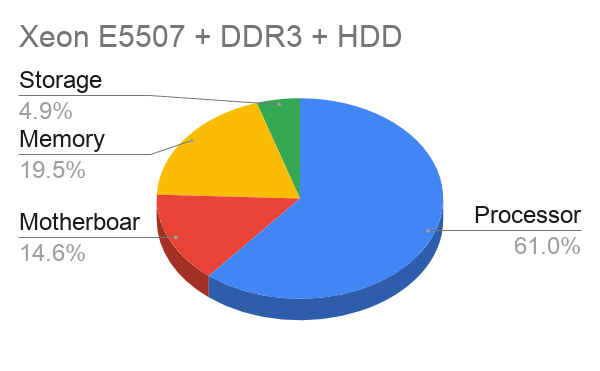
\includegraphics[width=\textwidth]{models/figures/power_breakdown/Xeon E5507 + DDR3 + HDD.png}
		\caption{}
		\label{fig:powerbreakdown_b}
	\end{subfigure}
	
	\hfill
	\caption{Power breakdown of a typical node of an HPC cluster at full use. The system used in this study (\textbf{a}) was built in 2016 and equipped with two Intel Xeon E5-2698, 128 GB of DDR4 memory and SSD as storage, while (\textbf{b}) the case study in \cite{Malladi2012TowardsDRAM} was built in 2012 and equipped with two Xeon E5507, 32GB of DDR3 memory and HDD as storage.}
	\label{fig:powerbreakdown}
\end{figure}

DVFS is motivated by the well-known fact that frequency and power have a near-cubic relationship \cite{Dayarathna2016DataSurvey, Group2012HandbookSahni}; this implies that running the CPU at a lower frequency causes a linear reduction in performance and a near-cubic reduction in power, which could lead to a near-square reduction in CPU energy.
Because of this, it is possible to achieve dramatic energy savings just with frequency control, depending on the system and its architecture.
Although very promising, the system software has yet to determine when and what voltage and frequency to use when running applications.
Otherwise, not only will performance deteriorate, but, in the worst case, energy consumption would also increase  \cite{Group2012HandbookSahni}.
Indeed, reducing the frequency results in a longer execution time, which increases the energy consumption of other system components, such as memory and disks.
There is also an overhead of time and energy associated with a voltage and frequency switch that needs to be considered.
Thus, finding the most appropriate voltage and frequency to use in all circumstances is not easy.
Therefore, since its introduction in 1994 \cite{Group2012HandbookSahni}, there has been a tremendous amount of research on DVFS algorithms.

The DPM technique can achieve substantial energy savings on systems where the static power is high, or the system remains inactive for a long time.
In that case, the problem is to determine when and which components to turn on/off.
With DPM, energy savings of 70\% have been reported~\cite{Shuja2012Energy-efficientCenters, Benini2000AManagement}. 

However, at the same time, while these power-saving techniques reduce system energy, they can compromise  performance leading  to a complex trade-off that needs to be carefully exploited to produce more energy-efficient algorithms.
Indeed, this study investigates whether the construction of an energy consumption model of an application can lead to significant energy savings.

We propose an analytical energy model for a given application in the function of the two control variables present in most HPC systems: CPU operating frequency and number of active cores. The model is composed of three application-dependent parameters and three parameters relating to the architecture of the system. The application parameters incorporate characteristics of the percentage of parallelism and the input size. The system architecture parameters include power-related and technology-dependent components, such as dynamic, static, and leakage power.

\section{Theoretical Background} \label{sec:theoretical_background}

A model is a formal representation of a natural system. The representation of computer system models includes equations, graphical models, rules, decision trees, representative collections of examples, and neural networks. The choice of representation affects the model's accuracy, as well as its interpretability by people~\cite{Hypothesis2012EncyclopediaLearning, Roy2019ForecastingNetwork, Zhu2019PredictingLearning}. Accurate energy and power consumption models are essential for many energy efficiency schemes employed in computing equipment \cite{Rivoire2007ModelsOptimizations}, and they can have multiple uses, including the design, forecasting, and optimization of data center systems. This study focuses on analytical models that could aid energy optimization and analyses of crucial factors in the total energy draw.

The desirable properties of a full-system model of energy consumption include accuracy, speed, generality and portability, inexpensiveness, and simplicity \cite{Rivoire2008AModels}. However, modeling an HPC system's exact energy consumption behavior is not straightforward, either at the whole-system level or at the level of individual components. Data centers' energy consumption patterns depend on multiple factors, such as hardware specifications, workload, cooling requirements, or the type of the applications. Some of these factors cannot be measured easily. Furthermore, it is impractical to perform detailed measurements of the energy consumption of lower-level components without additional overhead.

Several proposed models have already been classified concerning their input parameters, as shown by Dayarathna et al.~\cite{Dayarathna2016DataSurvey}, who analyzed more than 200 models according to their characteristics and limitations and classified them into categories where the model is more suited to its objectives:
\begin{itemize}
	%\item Temperature
	\item System utilization or workload
	\item Frequency
	\item Other system states, such as cache miss, branch prediction, number of instructions executed, and more
	\label{tab:input_type}
\end{itemize}

Often, energy models are described as a combination of two main parts, the power model of the system and the performance model of the application. This is because the concept of energy (E) is the total amount of work performed by a system over a period of time (T), while power (P) is the rate at which the system performs the work. The relation between these three amounts can be expressed as:
\begin{equation}
	E = \int_{0}^{T}P(t)dt.
	\label{eq:energy_definition_cont}
\end{equation}

\subsection{Power Models}

The modeling of system parameters is becoming popular nowadays with the advantage of performance counters provided by the CPU or the operating system. These counters can measure micro-architectural events, such as instructions executed, cache hits, miss-predicted branches, and more; thus, providing a base for many different estimations of power usage. This makes this type of model very suitable for power estimation because it can use information about several internal states of the computer.

Frequency-based models are the most common kind of model. They serve as a base for many power models~\cite{Sarwar1997CmosCalculation, Butzen2007LeakageGates, Usman2013ANoC}. These models utilize the fact that every digital circuit (including modern processors) is composed of transistors. Thus, modeling one transistor's interaction and scaling this to the chip can give a reasonable estimate of the entire system's energy. One of the most common frequency-based %please confirm that the intended meaning has been retained.
model approximations is defined as follows: 
\begin{equation}
	P = \alpha+\beta f^3,
	\label{eq:power_simplified}
\end{equation}
where $\alpha$ and $\beta$ are model parameters, and $f$ is the operating frequency (details of this equation are covered in (\cref{chapter:models}). This type of model is suitable for optimization problems since these are a function of the operating frequency, which can be easily controlled.

% We confirm that the meaning has been retained

\subsection{Performance Models}
The most common way to model the application performance is using the workload. The workload is an abstract representation of the amount of work done for a given time and speed. The workload ($W$) can be defined in many different ways. One common way, used in many studies, such as Paolillo et al. ~\cite{Paolillo2018OptimisationParallelism}, Francis et al. \cite{ Group2012HandbookSahni}, and Kim et al. \cite{Kim2015RacingHeuristics}, is the following:
\begin{equation}
	W = \int_{0}^{\tau}s(t)dt = s\tau,
	\label{eq:workload_definition}
\end{equation}
where $\tau$ is total active time, and $s$ is the execution speed in instructions/second.

Utilization models \cite{Fu2018RaceMinimization, Group2012HandbookSahni} are also found in the literature, defined as the ratio between the time that the system is active and the total time (idle and active). These models are present in many DVFS algorithms present in Linux. They can be viewed as a good alternative to the workload since it is impossible to measure workload in real-time.  \cref{eq:utilization_definition} defines workload in terms of CPU utilization ($u$):
\begin{equation}
	u = \frac{\tau}{T} = \frac{W/s}{T},
	\label{eq:utilization_definition}
\end{equation}
where $T$ is the total execution time (idle and active), and $\tau$ is the active time, meaning when the processor was executing instructions.
Models based on CPU utilization are the basis for DVFS algorithms. Even though this is not a controllable parameter, it is straightforward to measure system utilization with almost no overhead, and it is also very portable in terms of operating systems and architectures.

\section{Related work} \label{sec:related_work}

Merkel et al.~\cite{Merkel2006BalancingSystems} developed an energy model for processors based on events. Their model assumes a fixed energy consumption $\alpha_i$ for each activity, and by counting the number of occurrences $c_i$ of every activity, they estimate the total energy as:
\begin{equation}
	E = \sum_{i=1}^{n}\alpha_ic_i.
	\label{equation:rw_merkel}
\end{equation}

Another event-based model, introduced by Roy et al. \cite{Roy2013AnAlgorithms}, described the computational energy consumed by a CPU for an algorithm $A$ as the Equation (\ref{equation:rw_event_based})%\cref{equation:rw_event_based}:
\begin{equation}
	E(A) = P_{clk}T(A) + P_wW(A),
	\label{equation:rw_event_based}
\end{equation}
where $P_{clk}$ is a processor clock leakage power, $T(A)$ is the total execution time, $W(A)$ is the total time taken by  non-I/O operations, and $P_w$ is used to capture the power consumption per operation performed by the CPU. $T(A)$ and $W(A)$ are estimated using performance features.

Models based on events present some drawbacks, they are highly dependent on the operating system and its architecture, making them problematic to port for other platforms. There are also limitations regarding the number of simultaneous events that can coexist without adding a non-negligible overhead. Additionally, there are cases where events need multiplexing, for example, when using more hardware events than %please confirm that the intended meaning has been retained.
the CPU can provide. There are also some well know problems regarding the precision of some events, as shown in many studies~\cite{Weaver2008CanTrusted, Weaver2013Non-determinismImplementations, Das2019SoK:Security, McGuire2009AnalysisKernel, Ramos2019AnCounters, Silva-de-Souza2020ContainergyAWorkloads}. Some events that should be exact and deterministic (such as the number of executed instructions) show run-to-run variations and over-count on various architectures, even when running in strictly controlled environments. Because of that, our proposed model is not dependent on events and, therefore, not vulnerable to those drawbacks.
% We confirm that the meaning is the same

An instruction-level energy model was also proposed in \cite{Shao2013EnergyProcessor} by Yakun et. al. Where they proposed an energy per instruction (EPI) characterization made on Xeon Phi. Their model is expressed as:
\begin{equation}
	E(f) = \frac{(p_1 - p_0)(c_1 - c_0)/f}{N}, 
	\label{eq:rw_instruction_level}
\end{equation}
where $N$ is the total number of dynamic instructions, $p_0$ is the initial idle power, $p_1$ is the average dynamic power, and ($c_1$ $-$ $c_0$) refers to the cumulative number of cycles the micro-benchmark performs. This model is suitable for estimating the energy after the application finishes executing when it is possible to count the total cycles. However, it is challenging to use for optimization or forecasting since it does not have an application model to predict the cycles. Our model integrates the behavior of the application, taking into account the execution time.


Lewis et al.~\cite{Lewis2008Run-timeSystems} described the overall system energy consumption using the following equation:
\begin{equation}
	E = A_0(E_{proc} + E_{mem}) + A_1E_{em} + A_2E_{board} + A_3E_{hdd},
	\label{eq:lewvis}
\end{equation}
where, $A_0$, $A_1$, $A_2$, and $A_3$ are unknown constants that are calculated via linear regression analysis and those remain constant for a specific server architecture. This model, as the previous one, relies on knowledge of energy spent on each component, being  a suitable option for estimation after the application has already run, but not for optimization of the run itself, which is the aim of our model.

In another energy consumption model  based on system utilization, Mills et al. \cite{Mills2014EnergySystems} modeled the energy consumed by a compute node with CPU (single) executing at speed $\sigma$ as Equation (\ref{eq:mills})%\cref{eq:mills},
\begin{equation}
	E(\sigma,[t_1,t_2]) = \int_{t_1}^{t_2} \sigma^3 + \rho \sigma_max^3 dt,
	\label{eq:mills}
\end{equation}
where $\rho$ stands for the overhead power consumed regardless of the processor speed, $t_1$ and $t_2$ are the application's initial and final execution times. The overhead includes power consumption by all other system components, such as memory, network, and more. For this reason, although the authors mentioned the energy consumption of a socket, their power model is generalized to the entire server. This model lacks a closed-form, i.e., it depends on the definition of $\alpha(t)$ to be complete. Our model has a closed-form which facilitates analyses.


\subsection{The contribution of this work}

Although much work has been done on DVFS, the focus is still on the consumer electronics and laptop markets. 
For HPC, the notion of energy perception is relatively new~\cite{Feng2003MakingSupercomputing}. 
Moreover, the operational characteristics of non-HPC and HPC systems are significantly different. 
First, the workload on non-HPC systems is very interactive with the end-user, but the workload on the HPC platform is not.
Second, activities conducted on a non-HPC platform tend to share more machine resources.
In contrast, in HPC, each job often runs with dedicated resources. 
Third, an HPC system is usually much larger than a non-HPC system, making it more challenging to gather information, organize, and execute global decisions.
Therefore, it is worthwhile to investigate whether a DVFS scheduling algorithm, which works well for conventional computing, remains effective for HPC.

Our paper proposes a full-system energy model based on the CPU frequency and the number of cores. The model aims to understand and optimize the energy behavior of parallel applications in HPC systems according to application parameters, such as the degree of parallelism and CPU parameters related to dynamic and static power. The proposed model differs from existing ones, including the frequency and number of cores in the same equation for estimating the energy for a specific application in a given configuration. This model can serve as a base for considering DVFS and DPM optimization problems, including frequency and active cores. It can also be used to analyze the contribution of each parameter (ex: level of parallelism) to energy consumption. Furthermore, the number of cores is essential in HPC since applications are designed to run on multiple cores.

The proposed energy model is the product of an application-agnostic power model and an architecture-specific application performance model. The power model is based on the CMOS logic gates power draw as a function of the frequency~\cite{Sarwar1997CmosCalculation, Butzen2007LeakageGates} augmented to include the number of cores. The performance model is based on Amdahl's law \cite{Amdahl1967ValidityCapabilities, Eyerman2010ModelingDesign, Gustafson1988ReevaluatingLaw}, which can be used to estimate runtime in multi-core systems. In addition, this model has been extended to include execution frequency and input size, characterizing the application on the target architecture.


\cref{tab:related_work} summarizes the models comparing the system dependencies and the controllable variables.
\begin{table}[H]
	\footnotesize
	\caption{Related work summary.\label{tab1}}
	\setlength{\tabcolsep}{2.3mm}\begin{tabular}{cccc}
		\toprule
		%\begin{adjustwidth}{-\extralength}{0 cm}
		
		\textbf{Model}  & \textbf{System Dependency}       & \textbf{Variable}                     & \textbf{Controllable Variables}         \\ \midrule
		Merkel et al. \cite{Merkel2006BalancingSystems} & performance counters    & number of activities & - \\
		Roy et al. \cite{Roy2013AnAlgorithms}&performance counters &io operations, total time    & - \\
		Yakun et al. \cite{Shao2013EnergyProcessor}&number of instructions &frequency&frequency \\
		Lewis et al. \cite{Lewis2008Run-timeSystems}&energy of subcomponents&energy of subcomponents & - \\
		Mills et al. \cite{Mills2014EnergySystems}&power of subcomponents&total time, frequency & frequency \\ 
		Our model & - & frequency, cores, input size & frequency, cores, input size\\ \bottomrule
	\end{tabular}
	%\caption{Related work summary}
	\label{tab:related_work}
	%\bottomrule
\end{table}

%The main contributions of the proposed model are:
%
%\begin{itemize}
%	\item Simple model: faster to fit and compute, good for DVFS and DPM optimization.
%	\item Parameters with logical meaning: helps to understand the contribution of each specific term.
%	\item Analytical analysis: several analyses can be derived from the equation.
%	\item Controllable variables: the equation is in the function of parameters that we can control directly.
%\end{itemize}
